% ===== 07-mle =====
\section*{Maximum Likelihood Estimation (MLE)}
\begingroup
\setlist[itemize]{label=\raisebox{0.15ex}{\scriptsize$\bullet$}}

\subsection*{Probability vs.\ Likelihood}
Running example: flip a coin $N = 10$ times and get $n_1 = 7$ heads. $\mu$ = probability of heads.

\begin{itemize}
  \item \textbf{Probability:} $\mu$ is fixed, and we ask how likely the data is.\\
  Fair coin ($\mu = 0.5$): $P(\text{7 heads in 10} \mid \mu = 0.5) = \binom{10}{7}(0.5)^7(0.5)^3 \approx 0.117$.
  \item \textbf{Likelihood:} the data is fixed, and we ask how well each $\mu$ explains it.\\
  After seeing 7 heads: $L(0.7) \approx 0.267$ beats $L(0.5) \approx 0.117$.
\end{itemize}
\[
L(\mu) = p(\mathcal{D} \mid \mu) = \binom{10}{7}\,\mu^7 (1-\mu)^3
\]
\begin{itemize}
  \item Same formula, different variable: probability varies the data, likelihood varies $\mu$.
  \item \textbf{Probabilities sum to 1:} over all outcomes (0 to 10 heads), the bars add to 1.
  \item \textbf{Likelihoods don't:} over all $\mu$, $\int_0^1 L(\mu)\,d\mu = \tfrac{1}{11} \neq 1$. So $L(\mu)$ is \textbf{not} a distribution over $\mu$.
\end{itemize}

\begin{keeptogether}
{\centering
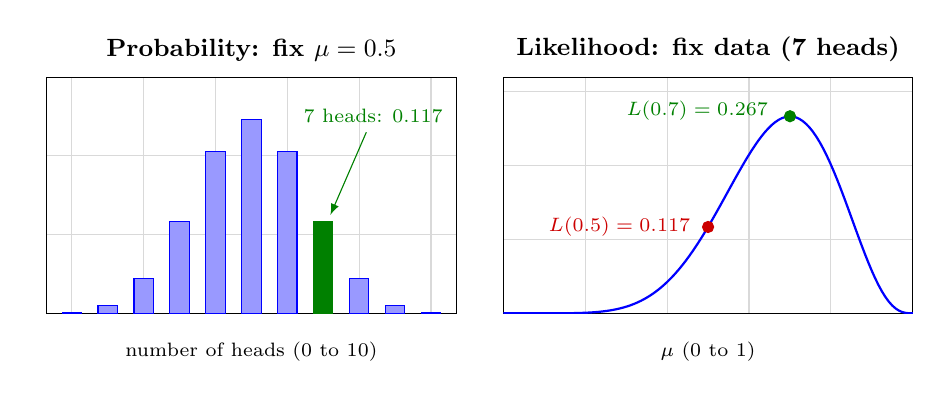
\begin{tikzpicture}
% ---- probability: vary the data ----
\begin{axis}[name=prob, scale only axis, width=5.2cm, height=3cm,
    xmin=-0.7, xmax=10.7, ymin=0, ymax=0.3, enlargelimits=false,
    grid=major, grid style={gray!30}, major tick length=0pt,
    xticklabels={}, yticklabels={},
    title={\small\textbf{Probability: fix $\mu = 0.5$}}, title style={yshift=-4pt},
    xlabel={\scriptsize number of heads (0 to 10)}, label style={font=\scriptsize}]
\addplot[ybar, bar shift=0pt, bar width=7pt, fill=blue!40, draw=blue] coordinates {
  (0,0.001) (1,0.010) (2,0.044) (3,0.117) (4,0.205) (5,0.246)
  (6,0.205) (8,0.044) (9,0.010) (10,0.001)};
\addplot[ybar, bar shift=0pt, bar width=7pt, fill=green!50!black, draw=green!50!black] coordinates {(7,0.117)};
\node[font=\scriptsize, green!50!black, anchor=south east] at (axis cs:10.6,0.23) {7 heads: 0.117};
\addplot[green!50!black, -latex] coordinates {(8.2,0.23) (7.2,0.125)};
\end{axis}
% ---- likelihood: vary mu ----
\begin{axis}[name=lik, at={(prob.east)}, anchor=west, xshift=0.6cm,
    scale only axis, width=5.2cm, height=3cm,
    xmin=0, xmax=1, ymin=0, ymax=0.32, enlargelimits=false,
    grid=major, grid style={gray!30}, major tick length=0pt,
    xticklabels={}, yticklabels={},
    title={\small\textbf{Likelihood: fix data (7 heads)}}, title style={yshift=-4pt},
    xlabel={\scriptsize $\mu$ (0 to 1)}, label style={font=\scriptsize}]
\addplot[thick, blue, domain=0:1, samples=120] {120*x^7*(1-x)^3};
\addplot[only marks, mark=*, red!80!black, mark size=2pt] coordinates {(0.5,0.117)};
\node[font=\scriptsize, red!80!black, anchor=east] at (axis cs:0.48,0.117) {$L(0.5) = 0.117$};
\addplot[only marks, mark=*, green!50!black, mark size=2pt] coordinates {(0.7,0.267)};
\node[font=\scriptsize, green!50!black, anchor=east] at (axis cs:0.67,0.275) {$L(0.7) = 0.267$};
\end{axis}
\end{tikzpicture}
\par}
\end{keeptogether}

\subsection*{What MLE Does}
\textbf{MLE = pick the parameter that maximizes the likelihood} (the peak of the curve):
\[
\mu_{\text{ML}} = \arg\max_{\mu} L(\mu) = \arg\max_{\mu} \ln L(\mu) = \frac{n_1}{N} = \frac{7}{10}
\]
\begin{itemize}
  \item In practice, maximize $\ln L(\mu)$: the product becomes a sum, and the peak is in the same place.
  \item The $\binom{10}{7}$ doesn't depend on $\mu$, so dropping it doesn't move the peak.
\end{itemize}

\begin{keeptogether}
{\centering
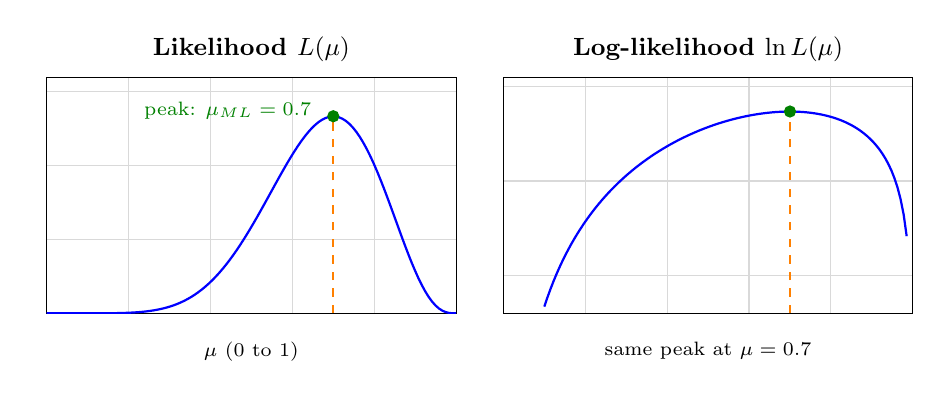
\begin{tikzpicture}
% ---- L(mu) ----
\begin{axis}[name=L, scale only axis, width=5.2cm, height=3cm,
    xmin=0, xmax=1, ymin=0, ymax=0.32, enlargelimits=false,
    grid=major, grid style={gray!30}, major tick length=0pt,
    xticklabels={}, yticklabels={},
    title={\small\textbf{Likelihood $L(\mu)$}}, title style={yshift=-4pt},
    xlabel={\scriptsize $\mu$ (0 to 1)}, label style={font=\scriptsize}]
\addplot[thick, blue, domain=0:1, samples=120] {120*x^7*(1-x)^3};
\addplot[orange, dashed, thick] coordinates {(0.7,0) (0.7,0.267)};
\addplot[only marks, mark=*, green!50!black, mark size=2pt] coordinates {(0.7,0.267)};
\node[font=\scriptsize, green!50!black, anchor=east] at (axis cs:0.67,0.275) {peak: $\mu_{\text{ML}} = 0.7$};
\end{axis}
% ---- ln L(mu) ----
\begin{axis}[name=lnL, at={(L.east)}, anchor=west, xshift=0.6cm,
    scale only axis, width=5.2cm, height=3cm,
    xmin=0, xmax=1, ymin=-12, ymax=0.5, enlargelimits=false,
    grid=major, grid style={gray!30}, major tick length=0pt,
    xticklabels={}, yticklabels={},
    title={\small\textbf{Log-likelihood $\ln L(\mu)$}}, title style={yshift=-4pt},
    xlabel={\scriptsize same peak at $\mu = 0.7$}, label style={font=\scriptsize}]
\addplot[thick, blue, domain=0.1:0.985, samples=120] {ln(120) + 7*ln(x) + 3*ln(1-x)};
\addplot[orange, dashed, thick] coordinates {(0.7,-12) (0.7,-1.32)};
\addplot[only marks, mark=*, green!50!black, mark size=2pt] coordinates {(0.7,-1.32)};
\end{axis}
\end{tikzpicture}
\par}
\end{keeptogether}
\endgroup